\section{Definition}

    A Cayley tree is a symmetric tree, constructed starting from a central node of degree $k$. Each node at distance $d$ from the central node has degree $k$, until we reach the nodes at distance $P$ that have degree one and are called leaves. From \cite{barabasi}.

    \begin{figure}[H]
        \centering
        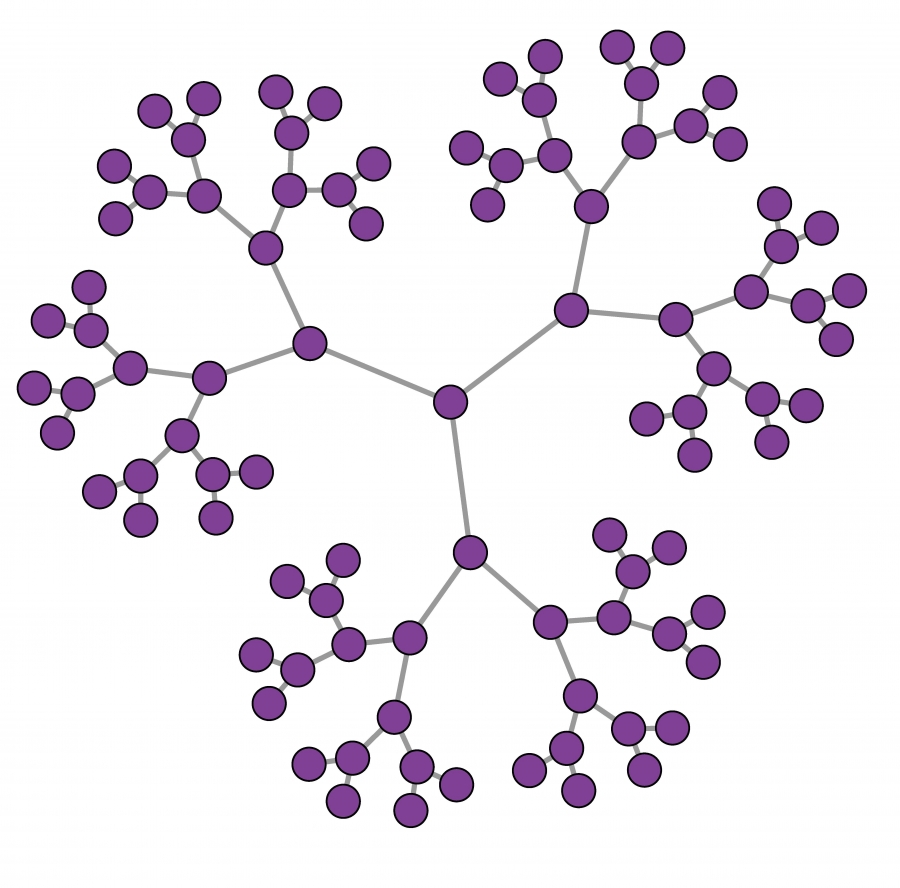
\includegraphics[width=0.5\textwidth]{images/caley-tree.jpg}

        \caption{Cayley tree with $k = 3$ and $P = 5$.}
    \end{figure}
